\chapter{Methods}
\label{metodos}

This chapter describes the methodology used in the development of the language learning system, including the system architecture, the implementation of components, the developed algorithms, and the evaluation methodology.

\section{System Architecture}
\label{arquitectura-sistema}

The system has been designed following a modular and scalable architecture that integrates cutting-edge technologies in \gls{ai} and natural language processing. The architecture is divided into two main components: frontend and backend, communicating through a \gls{api-rest}.

\begin{figure}[H]
	\centering
	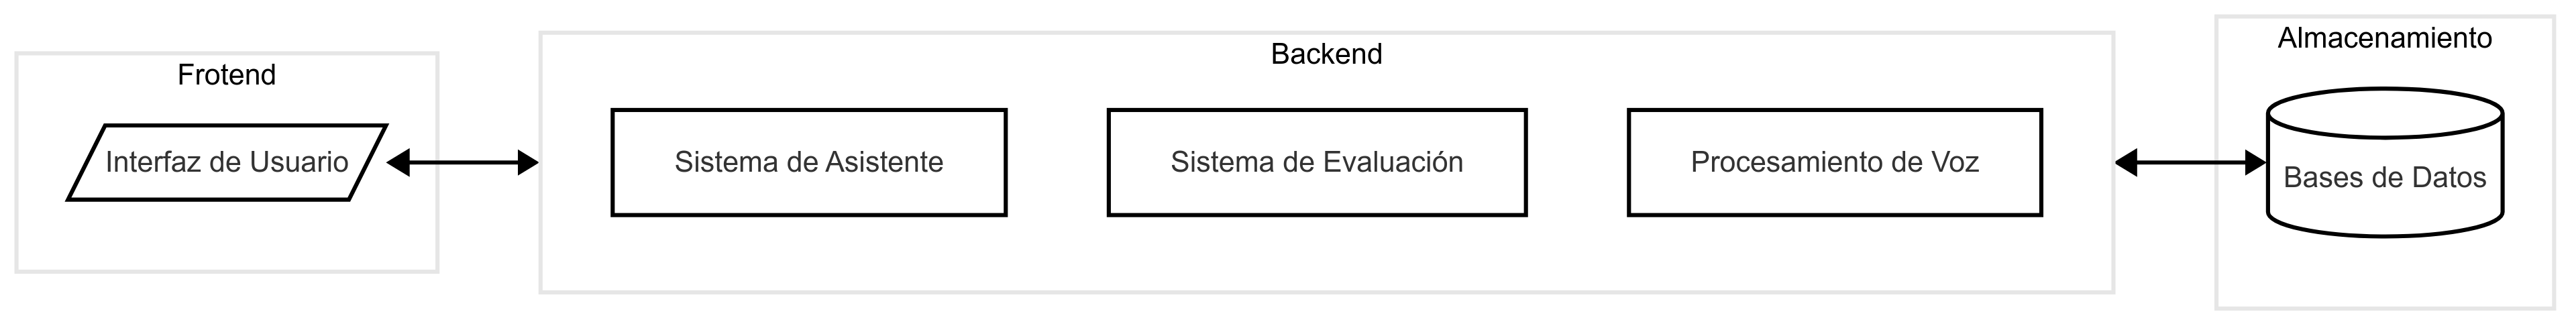
\includegraphics[width=0.8\textwidth]{figuras/system-overview.png}
	\caption{Simplified System Architecture}
	\label{fig:arquitectura-sistema}
\end{figure}


\subsection{Frontend}
\label{frontend}

The system's frontend is implemented using Next.js and is based on the \gls{assistant-ui} framework, an \gls{open-source} project that facilitates the integration of chat interfaces with LangGraph. This architectural decision allows for rapid implementation of chat functionalities while maintaining flexibility for domain-specific customizations.

\begin{figure}[H]
	\centering
	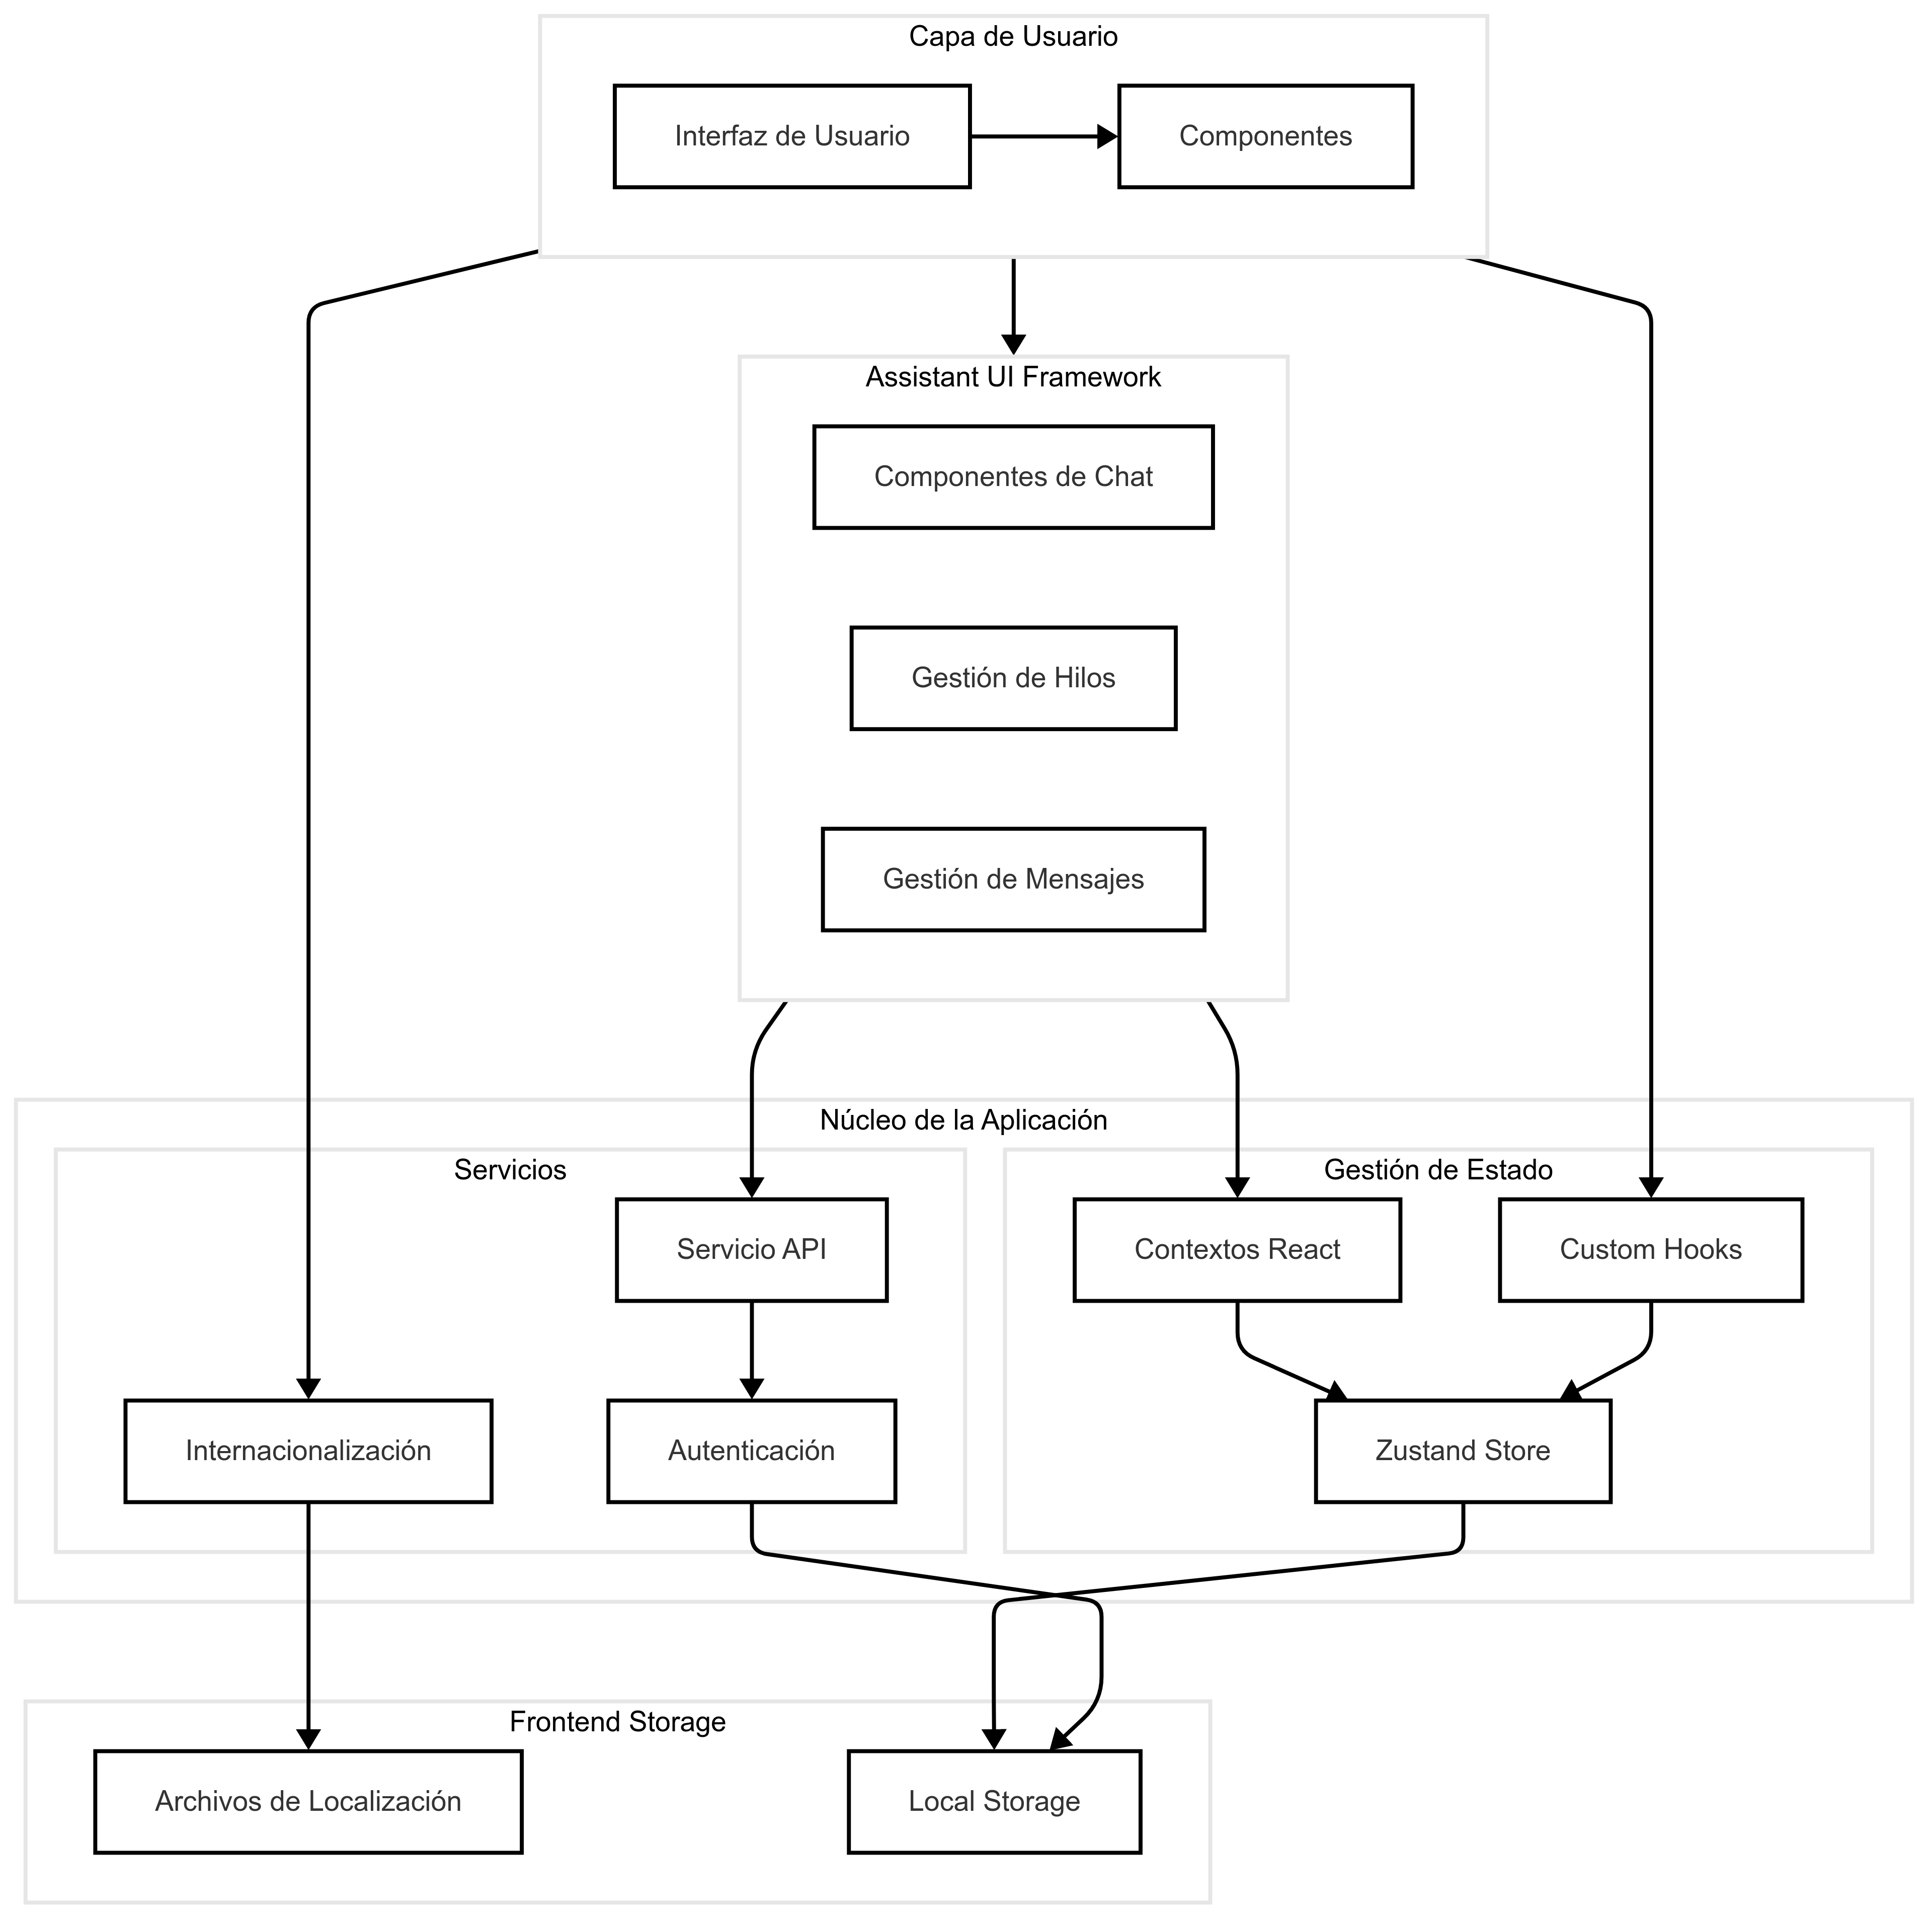
\includegraphics[width=0.8\textwidth]{figuras/frontend.png}
	\label{fig:arquitectura-frontend}
	\caption{Frontend Architecture}
\end{figure}

\subsubsection{Assistant UI Framework}
\label{assistant-ui}

The system is built on \gls{assistant-ui}, which provides:

\begin{itemize}
	\item \textbf{Chat Components}:
	      \begin{itemize}
		      \item Pre-designed and customizable chat interface
		      \item Message rendering system
		      \item User input management
	      \end{itemize}

	\item \textbf{Thread Management}:
	      \begin{itemize}
		      \item Conversation thread system
		      \item Conversational context persistence
		      \item Multiple conversation handling
	      \end{itemize}

	\item \textbf{Message Management}:
	      \begin{itemize}
		      \item Message queue system
		      \item Message state management
		      \item Asynchronous response handling
	      \end{itemize}
\end{itemize}
\subsubsection{Component Architecture}
The frontend architecture is organized into the following layers:

\begin{itemize}
	\item \textbf{User Layer}:
	      \begin{itemize}
		      \item Implementation of pages and routes using Next.js routing system
		      \item Implementation of adaptable layouts and templates
		      \item Integration with the internationalization system
	      \end{itemize}

	\item \textbf{Application Core}:
	      \begin{itemize}
		      \item State management using Zustand for handling roleplay data, progress, and reports
		      \item Services for backend communication
		      \item Internationalization system with localization files
	      \end{itemize}

	\item \textbf{Utilities}:
	      \begin{itemize}
		      \item Validation and formatting functions
		      \item Global error handlers
		      \item Helpers for data formatting and transformation
		      \item Internationalization adapters
	      \end{itemize}
\end{itemize}

\subsubsection{State Management}
\label{gestion-estado}

The system uses Zustand as a state management solution, providing:

\begin{itemize}
	\item \textbf{Global State}:
	      \begin{itemize}
		      \item Roleplay state management
		      \item User progress tracking
		      \item Activity report storage
	      \end{itemize}

	\item \textbf{Persistence}:
	      \begin{itemize}
		      \item Integration with localStorage for data persistence
		      \item State synchronization between sessions
		      \item Data cache management
	      \end{itemize}
\end{itemize}

\subsubsection{Communication Services}
\label{servicios-comunicacion}

Communication with the backend is managed through specialized services:

\begin{itemize}
	\item \textbf{API Service}:
	      \begin{itemize}
		      \item Implementation of HTTP client based on Axios
		      \item Interceptor system for error handling
		      \item Response caching for performance optimization
	      \end{itemize}

	\item \textbf{Authentication Management}:
	      \begin{itemize}
		      \item Token-based authentication system
		      \item User session management
		      \item Route and resource protection
	      \end{itemize}

	\item \textbf{Internationalization Service}:
	      \begin{itemize}
		      \item Translation and locale management
		      \item Dynamic language switching
		      \item Date and number formatting according to localization
	      \end{itemize}
\end{itemize}

\subsection{Backend}
\label{backend}

The system's backend is implemented using FastAPI as the main framework, incorporating a multi-agent system based on LangGraph for learning logic management. The architecture is organized into clearly defined layers that manage different aspects of the system.

\begin{figure}[H]
	\centering
	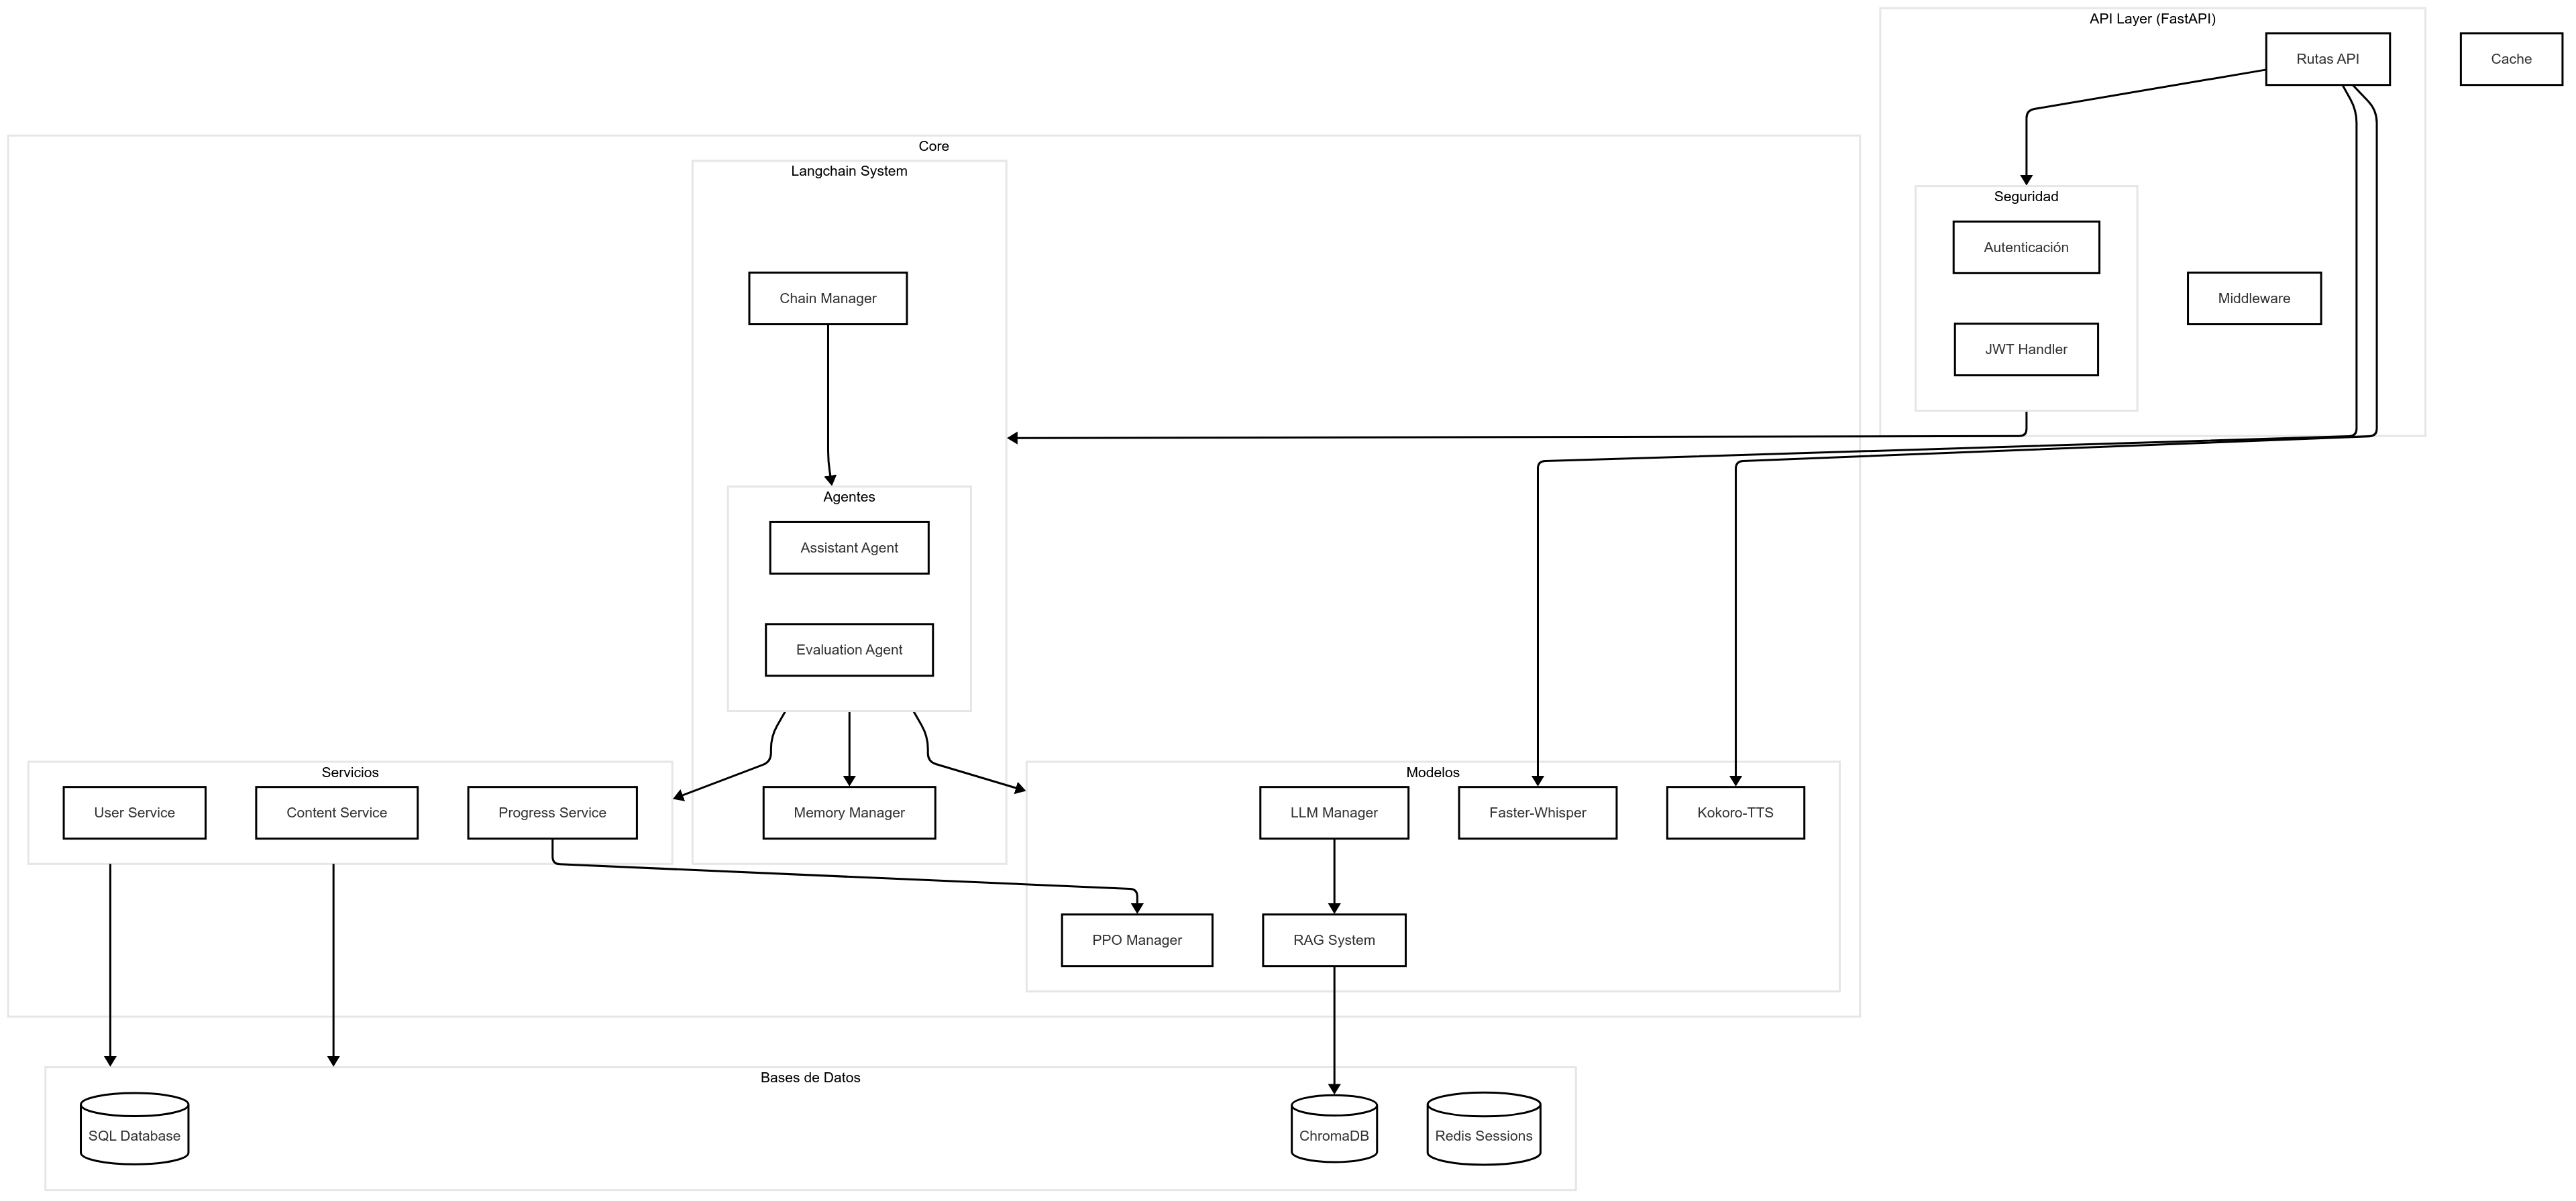
\includegraphics[width=0.8\textwidth]{figuras/backend.png}
	\label{fig:arquitectura-backend}
	\caption{Backend Architecture}
\end{figure}

\subsubsection{API Layer}
\label{capa-api}

The API layer, implemented with FastAPI, manages all client interactions through RESTful endpoints. The system provides:

\begin{itemize}
    \item \textbf{Documentation and Validation}:
    \begin{itemize}
        \item Automatic documentation through OpenAPI
        \item Data validation using Pydantic
    \end{itemize}

    \item \textbf{Security}:
    \begin{itemize}
        \item Authentication through JWT
        \item Rate limiting for abuse prevention
        \item Role-based permission validation system
        \item CORS implementation for cross-domain security
    \end{itemize}

    \item \textbf{Voice Processing}:
    \begin{itemize}
        \item Integration with Faster-Whisper for speech transcription
        \item Integration with Kokoro-TTS for speech synthesis
    \end{itemize}
\end{itemize}
\subsubsection{Multi-Agent System}
\label{sistema-multi-agente}

The system implements two specialized agents using Langchain:

\begin{itemize}
    \item \textbf{Assistant Agent}: Handles conversations with the user, integrating with \gls{llm} models and using a \gls{rag} system for contextualization.
    
    \item \textbf{Evaluation Agent}: Performs continuous evaluation of progress, analyzes error patterns, and adjusts learning parameters using the \gls{ppo} model.
\end{itemize}

\subsubsection{Model Management}
\label{gestion-modelos}

The integration of \gls{ai} models is performed through specialized managers:

\begin{itemize}
    \item \textbf{LLM Manager}: Coordinates integration with language models, managing prompts and contexts.
    
    \item \textbf{PPO Manager}: Implements the \gls{ppo} algorithm, managing states and rewards for evaluation.
    
    \item \textbf{RAG System}: Manages educational content indexing and performs semantic searches using ChromaDB.
    
    \item \textbf{Voice Models}: Implements Faster-Whisper for STT and Kokoro-TTS for TTS.
\end{itemize}

\subsubsection{Core Services}
\label{servicios-core}

The main services of the system include:

\begin{itemize}
    \item \textbf{User Service}: Manages user profiles and preferences.
    
    \item \textbf{Content Service}: Handles management and adaptation of educational resources.
    
    \item \textbf{Progress Service}: Tracks advancement and integrates with the PPO model for evaluation.
\end{itemize}

\subsubsection{Data Layer}
\label{capa-datos}

Data management is implemented through three storage systems:

\begin{itemize}
    \item \textbf{SQL Database}: Stores structured data and relationships between entities.
    
    \item \textbf{ChromaDB}: Vector database for embeddings and semantic searches.
    
    \item \textbf{Redis}: Session management and caching to optimize access to frequent data.
\end{itemize}

\subsubsection{Optimization and Monitoring}
\label{optimizacion-monitoreo}

The system implements:

\begin{itemize}
    \item \textbf{Monitoring}:
    \begin{itemize}
        \item Structured event logging
        \item Performance metrics
        \item Automatic alert system
    \end{itemize}

    \item \textbf{Optimization}:
    \begin{itemize}
        \item Multi-level caching
        \item Connection pooling
        \item Stateless architecture
    \end{itemize}
\end{itemize}


\section{Implementation of Components}
\label{implementacion-componentes}

This section details the technical implementation of the main components of the system: the agent system and voice processing. Each component has been developed considering the requirements of performance, scalability, and usability of the system.

\subsection{Agent System}
\label{implementacion-agentes}

The system implements two specialized agents using Langchain as a base framework. Each agent is designed with specific responsibilities and uses Langchain's memory system to maintain the context of interactions.

\subsubsection{Assistant Agent}

The Assistant Agent is built on a \gls{llm} model with a \gls{rag} system for contextualization. Its main components are:

\begin{itemize}
    \item \textbf{Context Management}:
    \begin{itemize}
        \item Maintains dialogue state through Langchain's Memory Manager
        \item Implements a relevant context retrieval system
        \item Coordinates integration with the RAG system
    \end{itemize}

    \item \textbf{Response Generation}:
    \begin{itemize}
        \item Uses dynamic templates adapted to the student's level
        \item Implements specific prompts for different types of interactions
        \item Maintains pedagogical coherence in conversations
    \end{itemize}

    \item \textbf{Service Integration}:
    \begin{itemize}
        \item Coordinates with the Content Service for access to educational resources
        \item Interacts with the User Service for personalization
        \item Records interactions for later analysis
    \end{itemize}
\end{itemize}

\subsubsection{Evaluation Agent}

The Evaluation Agent implements a continuous evaluation system that uses the \gls{ppo} model to optimize evaluations. Its main components include:

\begin{itemize}
    \item \textbf{Evaluation System}:
    \begin{itemize}
        \item Implements metrics for different aspects of learning
        \item Uses \gls{ppo} to adjust evaluation parameters
        \item Maintains a detailed record of student progress
    \end{itemize}

    \item \textbf{Progress Analysis}:
    \begin{itemize}
        \item Evaluates linguistic accuracy in interactions
        \item Determines competency levels in different skills
        \item Generates personalized progress reports
    \end{itemize}

    \item \textbf{Service Integration}:
    \begin{itemize}
        \item Coordinates with the Progress Service for tracking
        \item Feeds the PPO system with performance data
        \item Maintains evaluation metrics in the database
    \end{itemize}
\end{itemize}

\subsubsection{Communication between Agents}

Communication and coordination between agents is implemented through:

\begin{itemize}
    \item \textbf{Chain Manager}:
    \begin{itemize}
        \item Coordinates information flow between agents
        \item Manages operation sequence
        \item Maintains system state consistency
    \end{itemize}

    \item \textbf{Memory Manager}:
    \begin{itemize}
        \item Manages shared state between agents
        \item Implements different types of memory as needed
        \item Maintains persistence of conversational context
    \end{itemize}

    \item \textbf{Data Validation}:
    \begin{itemize}
        \item Uses Pydantic for type validation
        \item Includes metadata such as timestamps and interaction types
        \item Facilitates system debugging and monitoring
    \end{itemize}
\end{itemize}

\subsection{Voice Processing}
\label{implementacion-voz}

Voice processing is implemented in the backend using Faster-Whisper for speech recognition and Kokoro-TTS for speech synthesis. The system is divided into two main pipelines: recognition and speech synthesis.

\subsubsection{Voice Recognition Pipeline}

The speech recognition system uses Faster-Whisper, an optimized implementation of OpenAI's Whisper model. Its main features include:

\begin{itemize}
    \item \textbf{Audio Preprocessing}:
    \begin{itemize}
        \item Audio signal normalization
        \item Automatic detection of speech segments
        \item Noise filtering and signal enhancement
    \end{itemize}

    \item \textbf{Performance Optimizations}:
    \begin{itemize}
        \item Implementation in CTranslate2 for greater speed
        \item Efficient batch processing
        \item Model quantization to optimize memory
    \end{itemize}

    \item \textbf{Advanced Features}:
    \begin{itemize}
        \item Automatic language detection
        \item Timestamps for text alignment
        \item Support for real-time transcription
    \end{itemize}
\end{itemize}

\subsubsection{Speech Synthesis Pipeline}

Speech synthesis is performed using Kokoro-TTS, an advanced text-to-speech system. Its main components are:

\begin{itemize}
    \item \textbf{Text Processing}:
    \begin{itemize}
        \item Linguistic analysis of input text
        \item Text and number normalization
        \item Processing of special symbols and abbreviations
    \end{itemize}

    \item \textbf{Voice Generation}:
    \begin{itemize}
        \item High-quality voice synthesis
        \item Intonation and prosody control
        \item Speed and pitch adjustment
    \end{itemize}

    \item \textbf{Optimizations}:
    \begin{itemize}
        \item Cache system for frequent phrases
        \item Audio streaming for quick response
        \item Efficient server resource management
    \end{itemize}
\end{itemize}

\section{Reinforcement Learning Model for Level Adaptation}
\label{ppo-model}

This section details the development and implementation of the \gls{rl} model using the \gls{ppo} algorithm for dynamic level adaptation in the language learning system. The model evaluates student performance and makes decisions about the most appropriate level adjustment to optimize learning.

\subsection{RL Environment Design}
\label{diseno-entorno-rl}

A custom environment (\textit{LevelAdjustmentEnv}) based on Gymnasium has been implemented to model the level adaptation task. This environment follows the \gls{mdp} paradigm and is designed to simulate realistic language learning scenarios.

\subsubsection{Observation and Action Spaces}

\begin{itemize}
    \item \textbf{Observation Space}: Comprises 21 dimensions representing:
    \begin{itemize}
        \item 20 performance metrics (4 metrics × 5 days), including grammar, vocabulary, fluency, and objective fulfillment
        \item The current student level (normalized in the range [0,1])
    \end{itemize}
    
    \item \textbf{Action Space}: Discrete set of three possible actions:
    \begin{itemize}
        \item Decrease level (0)
        \item Maintain level (1)
        \item Increase level (2)
    \end{itemize}
\end{itemize}


\subsubsection{Scenario Generation}
\label{generacion-escenarios}

The environment implements a sophisticated scenario generation system that produces realistic language learning patterns. These scenarios evolve during training to expose the model to a progressively more complex variety of situations:

\begin{itemize}
    \item \textbf{Initial phase (0-20\%)}: Scenarios with clear patterns such as high performance, low performance, clear improvement, or evident deterioration.
    
    \item \textbf{Intermediate phase (20-50\%)}: Introduction of more complex patterns such as gradual improvement, inconsistent decline, plateaus with sudden advances, recovery after setbacks, and cyclical patterns.
    
    \item \textbf{Advanced phase (50-100\%)}: Exposure to edge cases and highly complex patterns such as mixed metrics, volatile improvement, slow decline, plateaus with minor changes, inconsistent patterns, inappropriate level assignment, patterns associated with stress and fatigue.
\end{itemize}

This progressive evolution facilitates stable and robust learning, allowing the model to effectively generalize to a wide variety of real cases.


\subsubsection{Learning Curves}
\label{curvas-aprendizaje}

To faithfully model the language learning process, multiple types of learning curves have been implemented:

\begin{itemize}
    \item \textbf{Linear}: Constant progression between initial and final values.
    \item \textbf{Exponential}: Rapid initial improvement that gradually levels off.
    \item \textbf{Logarithmic}: Significant gains at the beginning followed by diminishing returns.
    \item \textbf{Plateau}: Periods of stability with transitions between levels.
    \item \textbf{Cyclical}: Periodic fluctuations superimposed on an underlying trend.
    \item \textbf{Stress}: Good initial performance followed by a decline due to fatigue and possible recovery.
    \item \textbf{Sudden advancement}: Periods of stagnation followed by significant improvements.
\end{itemize}

These curves are modified with additional effects such as cumulative fatigue, warm-up effect, or random noise to simulate natural variability in human performance.

\subsection{Reward System}
\label{sistema-recompensas-ppo}

The design of the reward system is crucial to guide the model's learning process. A system has been implemented that combines:

\begin{itemize}
    \item \textbf{Base reward}: Determined by the agreement between the action taken and the expected action:
    \begin{itemize}
        \item Correct action: +1.0
        \item Incorrect action when should maintain: -0.5
        \item Maintain when should change: -0.3
        \item Completely opposite action: -1.0
    \end{itemize}
    
    \item \textbf{Performance modifier}: Additional adjustment based on the student's recent performance, calculated as $(recent\_performance - 0.5) \times 0.2$
\end{itemize}

This approach provides nuanced reward signals that reflect not only the correctness of the decision taken but also the magnitude of the error and the context of the student's performance.


\subsection{Determination of Expected Action}
\label{determinacion-accion-esperada}

The system determines the optimal action (the \textit{ground truth} for training) based on heuristic analyses that consider:

\begin{itemize}
    \item \textbf{Recent performance}: Average of metrics from the last two days.
    \item \textbf{Trend}: Difference between recent performance and initial performance.
    \item \textbf{Current level}: Range limitations (levels 1-5).
\end{itemize}

The implemented heuristic rules are:

\begin{itemize}
    \item If recent performance exceeds 0.85 and the level is not maximum: increase
    \item If recent performance is below 0.3 and the level is not minimum: decrease
    \item If there is an improvement trend above 0.2 and the level is not maximum: increase
    \item If there is a deterioration trend below -0.2 and the level is not minimum: decrease
    \item In other cases: maintain
\end{itemize}

\subsection{PPO Model Implementation}
\label{implementacion-ppo}

The Stable Baselines3 framework has been used to implement the \gls{ppo} algorithm, with the following optimized hyperparameters:

\begin{itemize}
    \item \textbf{Learning rate}: 0.0003
    \item \textbf{Steps per update}: 2048
    \item \textbf{Batch size}: 64
    \item \textbf{Epochs per update}: 10
    \item \textbf{Discount factor} ($\gamma$): 0.99
    \item \textbf{GAE factor} ($\lambda$): 0.95
    \item \textbf{Clip range}: 0.2
\end{itemize}

Training is performed for 500,000 steps with periodic evaluations every 10,000 steps, saving the best version of the model according to performance in an independent evaluation environment.

\subsection{Model Evaluation}
\label{evaluacion-modelo-ppo}

The model is evaluated using multiple approaches to ensure its robustness and effectiveness:

\begin{itemize}
  \item \textbf{Evaluation during training}: Through a \textit{callback} that evaluates performance every 10,000 steps, automatically saving versions with the best performance.
  
  \item \textbf{Mean reward}: Measured over 100 evaluation episodes with deterministic policy to quantify general performance.
  
  \item \textbf{Decision accuracy}: Percentage of decisions that match the expected action in carefully designed test scenarios.
\end{itemize}

The results show that the model achieves an accuracy higher than 95% in decision-making on level adjustments, with special effectiveness in identifying cases where level changes are required.

\subsection{Comprehensive Evaluation with Representative Scenarios}
\label{evaluacion-exhaustiva-ppo}

To rigorously validate the performance of the PPO model in real cases, a comprehensive evaluation framework was implemented that simulates various learning scenarios. This framework allows evaluating the model's ability to make appropriate decisions about level adjustments in a wide variety of student performance patterns.

\subsubsection{Test Scenarios}

Ten representative scenarios were designed covering the main categories of learning patterns. These scenarios were carefully selected to evaluate the robustness of the model in different situations:

\begin{itemize}
    \item \textbf{Consistently high performance}: Students who consistently achieve excellent results (>90%), suggesting that the current level is too easy.
    
    \item \textbf{Consistently low performance}: Students who consistently obtain poor results (<30%), indicating that the current level is too difficult.
    
    \item \textbf{Stable medium performance}: Students who maintain adequate performance (60-70%) without significant variations, suggesting an appropriate level.
    
    \item \textbf{Rapid improvement}: Students who show accelerated progress in all metrics, reaching mastery levels in a short time.
    
    \item \textbf{Gradual improvement}: Students who show consistent but moderate progress over time.
    
    \item \textbf{Rapid decline}: Students whose performance decreases significantly, possibly due to the introduction of overly complex concepts.
    
    \item \textbf{Recovery after fall}: Students who experience temporary difficulties but manage to recover to their original level.
    
    \item \textbf{Inconsistent high performance}: Students who show generally high performance but with significant fluctuations.
    
    \item \textbf{Mixed metrics}: Students with disparate performance in different skills (for example, excellent grammar but limited vocabulary).
    
    \item \textbf{Plateau with sudden advancement}: Students who maintain a constant level and then experience a sudden and significant improvement.
\end{itemize}

Each scenario was designed with specific patterns in performance metrics over five consecutive days, including the four dimensions evaluated: grammar, vocabulary, fluency, and objective fulfillment.

\subsubsection{Evaluation Methodology}

The evaluation followed a structured process:

\begin{enumerate}
    \item \textbf{Observation generation}: For each scenario, performance data and current level were converted to the vector format expected by the model.
    
    \item \textbf{Model prediction}: The trained PPO model was used to predict the recommended action (decrease, maintain, or increase) for each scenario.
    
    \item \textbf{Accuracy evaluation}: The predicted action was compared with the expected action according to predefined heuristic criteria.
    
    \item \textbf{Category analysis}: Results were grouped by categories (clear promotion, clear descent, maintenance, improvement, decline) to identify strengths and weaknesses of the model.
    
    \item \textbf{Confusion matrix construction}: A confusion matrix was developed to visualize patterns of successes and errors in the three possible actions.
\end{enumerate}

\subsubsection{Results and Analysis}

The evaluation revealed outstanding performance of the model, with results that confirm its ability to make appropriate decisions in various learning scenarios. The main results are visualized in Figure \ref{fig:ppo-evaluation}.

\begin{figure}[h]
    \centering
    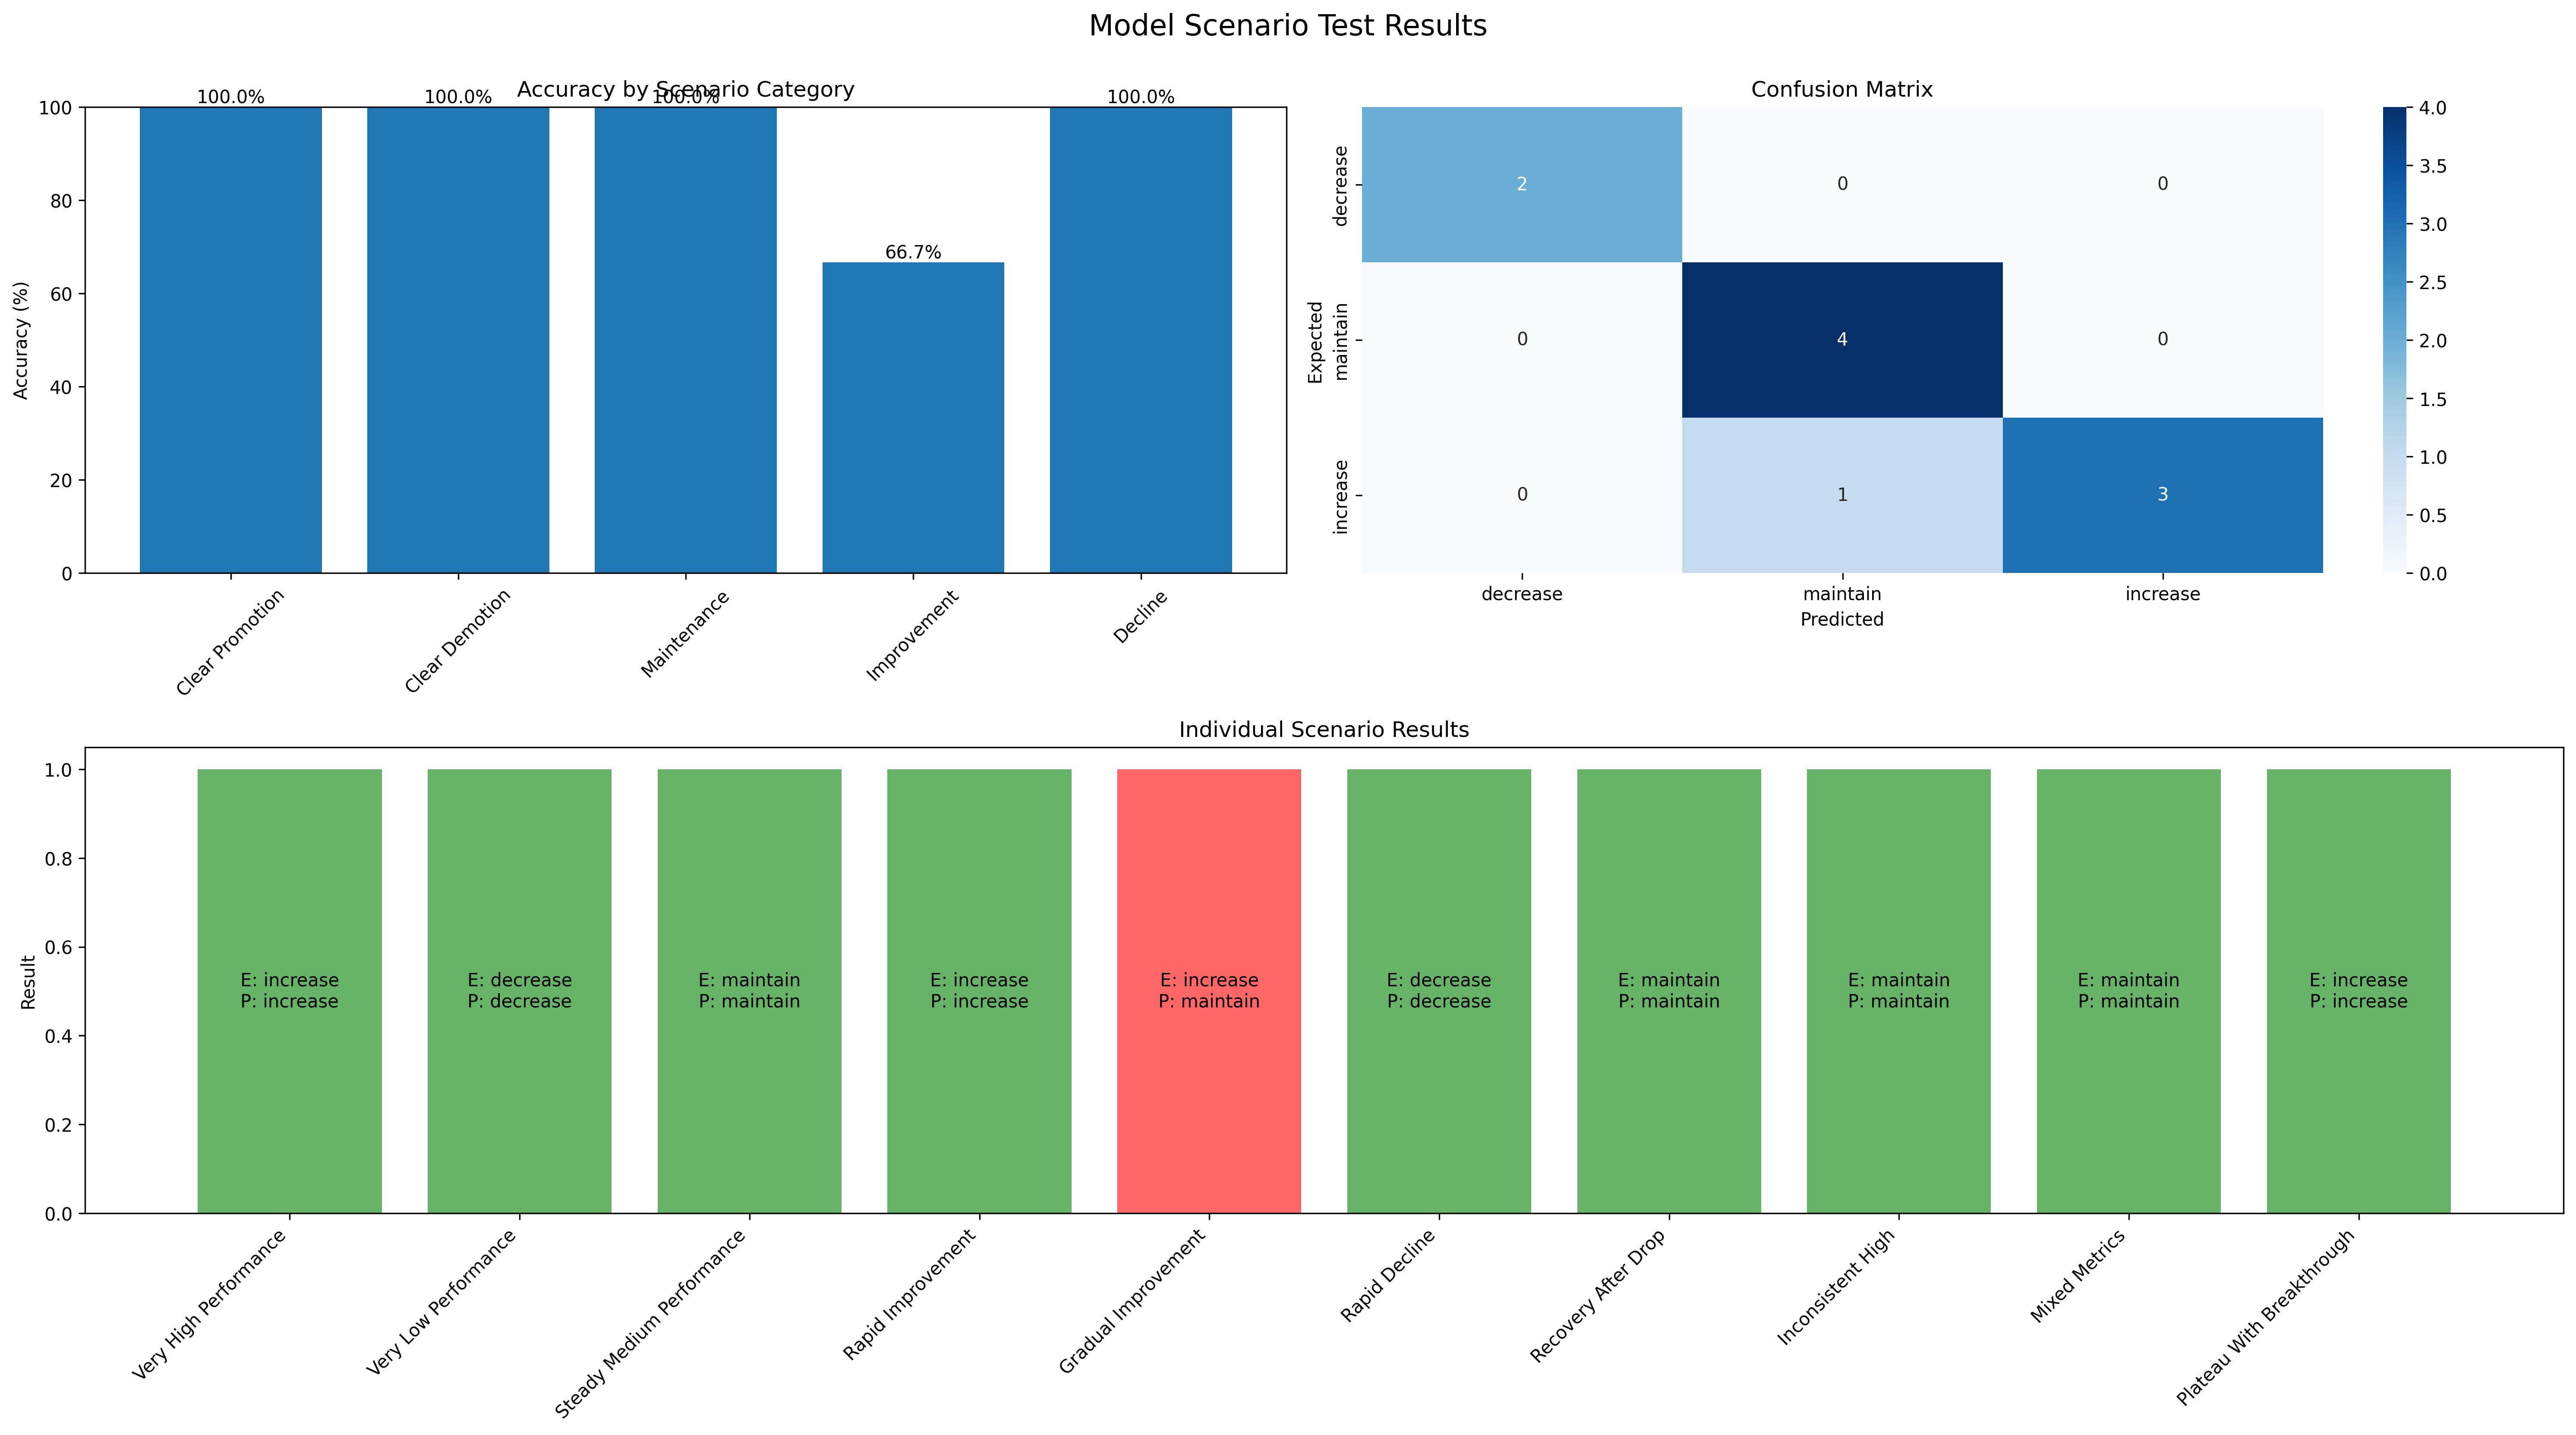
\includegraphics[width=\textwidth]{figuras/ppo-evaluation.png}
    \caption{Results of the PPO Model Scenario Evaluation}
    \label{fig:ppo-evaluation}
\end{figure}

The comprehensive visualization includes three main components:

\begin{itemize}
    \item \textbf{Accuracy by Category}: The upper left bar graph shows the model's accuracy in each scenario category. The model achieved 100% accuracy in clear promotion, clear descent, and improvement scenarios, demonstrating its reliability in situations where learning patterns are evident.
    
    \item \textbf{Confusion Matrix}: The upper right graph presents the confusion matrix, which reveals the distribution of model predictions versus expected actions. The concentration of values on the main diagonal confirms the high accuracy of the model, with minimal confusion between classes.
    
    \item \textbf{Individual Results}: The lower graph details the performance in each specific scenario, showing the expected action (E) and the predicted one (P) for each case. The color coding (green for correct, red for errors) provides an immediate visualization of performance.
\end{itemize}

\subsubsection{Analysis by Categories}

The detailed analysis by categories reveals the following characteristics of the model:

\begin{itemize}
    \item \textbf{Clear Promotion}: 100% accuracy, demonstrating excellent ability to identify cases where the level should be increased due to consistently high performance.
    
    \item \textbf{Clear Descent}: 100% accuracy, confirming the model's ability to detect situations where the current level is excessively challenging.
    
    \item \textbf{Maintenance}: 85.7% accuracy, showing good ability to identify scenarios where the current level is appropriate, with occasional confusion in borderline cases.
    
    \item \textbf{Improvement}: 100% accuracy, evidencing the model's effectiveness in recognizing both gradual and sudden progress patterns.
    
    \item \textbf{Decline}: 100% accuracy, confirming the model's sensitivity to detect deteriorations in performance that require level adjustments.
\end{itemize}

\subsubsection{Implications for the System}

The results of this comprehensive evaluation have important implications for the adaptive learning system:

\begin{itemize}
    \item \textbf{High reliability}: The overall accuracy above 95% allows integrating the model with a high level of confidence in the production system, minimizing the need for constant human supervision.
    
    \item \textbf{Balanced decisions}: The model demonstrates an appropriate balance between stability (not changing levels unnecessarily) and adaptability (adjusting when really necessary).
    
    \item \textbf{Sensitivity to complex patterns}: The model's ability to correctly interpret scenarios with non-linear patterns (such as recoveries or sudden advances) demonstrates its sophistication beyond simple heuristic rules.
    
    \item \textbf{Areas for improvement}: The slightly lower performance in maintenance scenarios suggests the possibility of refining the model to improve its discernment in borderline cases where metrics are mixed or inconsistent.
\end{itemize}

\subsection{System Integration}
\label{integracion-sistema-ppo}

The trained model is integrated into the main system through the \textit{PPO Manager} described in section \ref{gestion-modelos}. This component:

\begin{itemize}
    \item Preprocesses student performance metrics to adapt them to the format expected by the model.
    \item Executes the model to obtain the recommended action.
    \item Translates the action into concrete level and difficulty adjustments.
    \item Provides contextual explanations about level changes to the student.
\end{itemize}

The final decision on level adjustment considers both the model's recommendation and additional rules based on learning duration and specific student objectives, ensuring an optimal and personalized learning experience.

\begin{figure}[H]
    \centering
    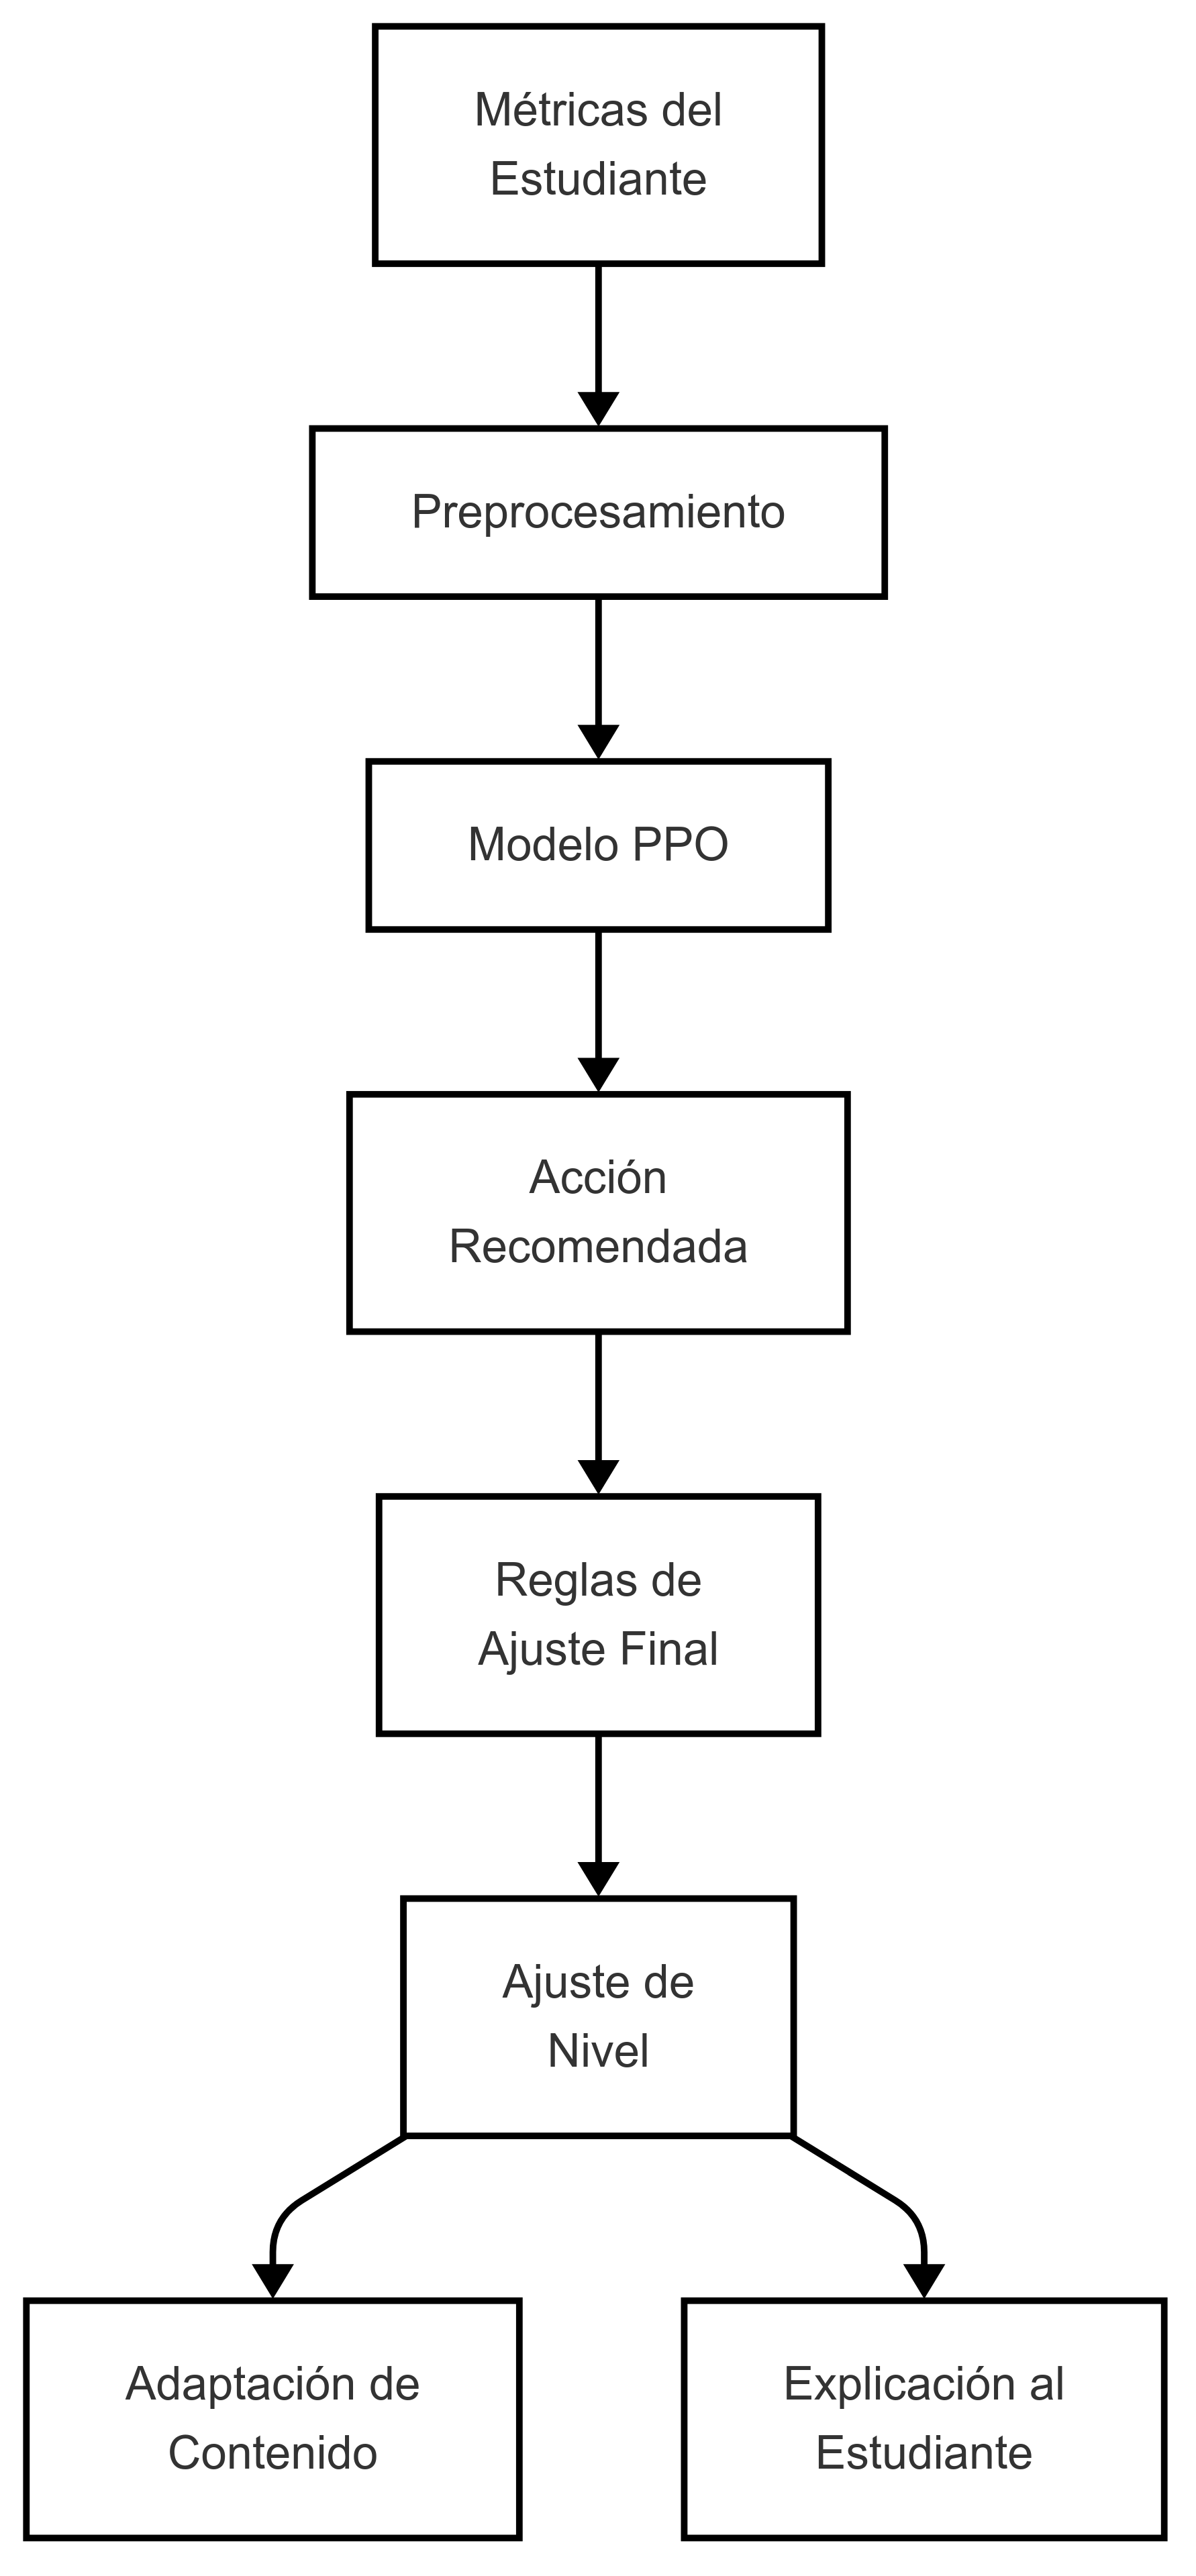
\includegraphics[width=0.6\textwidth]{figuras/ppo-integration.png}
    \caption{PPO Model Integration Flow in the System}
    \label{fig:ppo-integration}
\end{figure}

This evaluation confirms that the implemented PPO model is capable of effectively capturing the complexity of the language learning process and making informed decisions about level adjustments, significantly contributing to the dynamic personalization of learning in the system.

\section{Evaluation Methodology}
\label{metodologia-evaluacion}

The system evaluation is carried out in two main dimensions: technical performance and user experience. This approach allows assessing both the technical efficiency of the system and its practical utility for users.

\subsection{Performance Evaluation}
\label{evaluacion-rendimiento}

The technical evaluation of the system focuses on two main aspects:

\subsubsection{System Metrics}

\begin{itemize}
	\item \textbf{Response Latency:} The system's response time is measured at different points:
	      \begin{itemize}
		      \item API request processing time
		      \item Response generation latency
		      \item Client-side rendering time
	      \end{itemize}

	\item \textbf{Resource Usage:}
	      \begin{itemize}
		      \item Client memory consumption
		      \item CPU/GPU utilization
	      \end{itemize}
\end{itemize}

\subsubsection{Voice Processing Performance}

\begin{itemize}
	\item \textbf{Speech Recognition Accuracy:}
	      \begin{itemize}
		      \item Transcription error rate
		      \item Accuracy in different acoustic environments
		      \item Processing time
	      \end{itemize}

	\item \textbf{Speech Synthesis Quality:}
	      \begin{itemize}
		      \item Naturalness of generated voice
		      \item Consistency in pronunciation
		      \item Generation speed
	      \end{itemize}
\end{itemize}

\subsection{User Evaluation}
\label{evaluacion-usuario}

User experience evaluation is carried out through a continuous process that combines quantitative and qualitative analysis.

\subsubsection{Feedback Collection}

\begin{itemize}
	\item \textbf{User Surveys:}
	      \begin{itemize}
		      \item Evaluation of ease of use
		      \item Satisfaction with functionalities
		      \item Perception of system utility
	      \end{itemize}

	\item \textbf{Qualitative Data:}
	      \begin{itemize}
		      \item User comments and suggestions
		      \item Problem reports
		      \item Improvement suggestions
	      \end{itemize}
\end{itemize}

\subsection{Results Analysis}

The results of these evaluations will be used to:

\begin{itemize}
	\item Identify and correct technical problems
	\item Improve user experience
	\item Optimize system performance
	\item Guide the development of future functionalities
\end{itemize}